\chapter{引言}
\section{研究背景与意义}
随着全球金融市场电子化、自动化和机构化程度不断提高，对冲基金交易已经从依赖经验判断的投资活动，逐步演化为由数据处理、模型推断、组合配置、订单执行和风险反馈共同支撑的复杂决策系统。不同于单一价格预测任务，对冲基金交易需要在多资产、多空博弈、高杠杆约束和严格执行成本共同作用下持续形成可执行的交易判断，其结果不仅取决于模型能否识别价格方向，还取决于信号能否在资金配置、因子解释、时机识别和交易执行中保持一致。已有执行优化研究说明，交易指令的路径选择会影响策略收益能否在真实市场中兑现\cite{ning2021double}。这一结论对本文的启示在于，交易算法的评价不能停留在预测端，而必须向真实市场中的订单执行和收益兑现延伸。也就是说，模型输出只有经过可执行路径检验，才可能成为有效交易决策的一部分。交易信号真实性、方向判断和执行效果并非确定性输出，而是需要在概率意义上评估其可靠性\cite{qiao2026probability}。在本文看来，对冲基金交易中的算法问题并不是“预测模块越复杂越好”的单点优化问题，而是要判断预测信号能否沿着配置、解释、识别、执行和反馈环节连续传递，并最终形成可以落地的交易动作。因此，本文将对冲基金交易理解为一条连续的交易决策链，而不是孤立的预测模型优化问题；后续各章也围绕这一决策链依次展开。

在这一决策链中，首先涉及的是资产配置对象选择与资金配置问题。对冲基金通常同时面对股票、期货及其他衍生品等多类可交易对象，资产之间的相关性结构会随市场状态变化而改变，单一资产预测结果难以直接转化为稳定的资金配置方案。这里需要关注的并不是单个资产的预测误差，而是多个资产在同一资金约束下如何形成相对稳定的配置关系。多变量时间序列表征学习研究说明，长程依赖关系和跨变量交互是复杂时序建模中的重要问题\cite{zerveas2021transformer}。本文引用这一类研究，并不是将资产配置简单等同于多变量预测，而是强调对冲基金交易中的资产关系、资金约束和策略模块之间都具有动态交互特征。换言之，资产配置环节承担的是交易系统的入口功能：它决定哪些资产被纳入后续分析，也决定后续因子解释、结构识别和执行优化所面对的资金约束边界。若组合管理环节不能稳定刻画资产之间的相对强弱和风险约束，后续因子分析、时机识别和执行优化都可能建立在不稳定的配置基础上。

在明确资产配置对象之后，交易系统还需要形成稳定的因子依据，即从多维金融变量中识别能够支撑交易判断的信息。金融时序去噪与分类方法表明，在高噪声市场环境下，信号提取质量会影响后续方向判断与趋势识别\cite{liu2024denoising}。如果底层因子或信号被噪声主导，后续无论采用组合优化还是执行优化，都可能只是放大这种误差。由此，高维金融因子建模不应被视为单纯的特征工程，而应承担从高维、非平稳、弱信号数据中筛选有效信息的作用，为资产选择和后续策略判断提供依据。

当资产对象与因子依据初步形成后，交易系统进一步进入交易时机判断环节。金融市场价格序列并不只包含方向变化，还包含趋势延续、局部反转、结构破坏和噪声扰动等多种状态。深度序列模型已经被用于刻画金融市场中的非线性时序关系\cite{fischer2018deep}，但较强的拟合能力并不等同于稳定的交易时机识别能力；若缺乏结构化约束，模型仍容易将局部噪声误认为有效趋势。生成对抗网络（Generative Adversarial Network, GAN）为分布层面的样本生成与对抗式训练提供了基础范式\cite{goodfellow2014generative}。将这一思想引入金融时序结构识别时，需要进一步结合金融市场的非平稳性、厚尾特征和趋势结构约束，才能服务于交易时机判断。

交易信号进入市场之后，还必须进一步处理交易执行路径优化问题。高频交易相关研究表明，市场参与者的交易速度与订单行为会改变市场微观结构，从而影响策略执行结果\cite{ba2019highfreq}。这意味着算法交易系统面对的不是被动数据对象，而是会因交易行为发生变化的动态环境。大资金容量带来的流动性瓶颈与市场冲击成本，是制约对冲基金实盘表现的重要因素；即便预测方向基本正确，如果仓位规模、执行路径和市场流动性不匹配，策略收益也可能在交易过程中被滑点和冲击成本侵蚀。金融机器学习从理论训练走向真实应用时，还需要同时面对交易成本、风险暴露与市场约束等问题\cite{dixon2020machine}。因此，执行优化不能被视为预测之后的附属步骤，而应成为交易决策链中的关键环节。本文后续将交易执行单独作为一章处理，正是因为执行环节会把前序模型输出重新置于真实市场摩擦之中检验，只有当信号能够通过执行约束，理论收益才可能转化为可实现收益。

上述环节最终需要统一到最终交易判断与策略整合过程之中。已有金融时序预测综述表明，预测模型、特征学习和交易任务之间通常并非彼此孤立，而是共同构成算法交易系统的多个环节\cite{sezer2020financial_timeseries_review}。对冲基金交易中的最终判断并不是简单给出上涨或下跌标签，而是要在资产配置、因子依据、结构信号和执行约束之间形成一致的买入、卖出或持有决策。多智能体系统为这种复杂关系提供了建模基础，相关研究表明，在多个主体共同参与的系统中，协作、竞争与信息传递会影响系统稳定性和策略演化结果\cite{liang2020multiagent}。本文采用多智能体对抗学习，并不是为了在传统预测模型外部简单叠加一个智能体模块，而是希望利用智能体之间的交互、竞争和校验关系，将金融交易中的多主体博弈结构转化为可训练的模型关系。因此，本文将多智能体对抗学习作为贯穿全文的方法基础，目的在于通过系统内部的交互机制刻画金融市场中的多主体博弈关系。

区别于公募基金等传统买方机构，对冲基金的交易活动通常涉及做空机制、杠杆应用以及复杂衍生品交易。多空博弈要求算法不仅能识别价值增长，也要在下行市场中具备对抗性的信号捕捉能力；杠杆工具会同时放大收益和风险，对模型稳健性与实时风险控制提出更高要求；复杂衍生品与高维资产空间则进一步增加了非线性建模难度。从智能体建模角度看，多智能体深度强化学习在算法交易中的应用也表明，不同交易主体之间的交互会改变策略学习过程\cite{shavandi2022multiagent}。这说明交易系统中的主体关系并非外在背景，而会直接影响策略学习的方向、稳定性和最终结果。对于对冲基金而言，模型、资产、执行通道和风险约束之间同样存在相互作用，因而需要从系统层面组织算法结构。国内关于深度强化学习算法交易的综述进一步指出，交易策略不仅需要预测价格变化，还必须考虑仓位管理、交易成本与执行约束\cite{ning2020survey}。这些特征共同决定了对冲基金交易算法不能停留在单模型预测层面，而需要从系统角度组织研究对象。

从行业发展看，以文艺复兴科技（Renaissance Technologies）为代表的量化对冲基金，较早将数学建模、统计推断和计算方法引入交易决策。随着深度学习、大模型和强化学习技术不断发展，金融市场中的算法复杂度和算力投入持续提升。不过，通用模型训练研究提示，单纯扩大模型规模并不必然解决任务适配问题\cite{hoffmann2022training}。这一结论对本文的启示在于，金融交易算法不能把模型规模视为唯一改进方向。对冲基金交易更需要把模型能力放回资产配置、风险控制、交易成本和执行约束之中检验，否则模型复杂度提升未必能够转化为稳定收益。人工智能方法进入量化投资后仍需与具体交易约束相结合\cite{he2024ai}。如图~\ref{fig:1-1} 所示，对冲基金行业的算法化演进经历了从规则驱动到统计套利、再到深度算法与多智能体对抗学习阶段，这一演进路径表明，对冲基金交易场景对算法的博弈性、自适应性和稳健性具有较强内在需求。

\begin{figure}[htbp]
    \centering
    \includegraphics[width=0.9\textwidth]{figures/p1-1.pdf}
    \caption{对冲基金行业算法化演进与AI技术渗透路径}
    \label{fig:1-1}
\end{figure}

从方法发展看，深度学习为复杂非线性表征提供了基础\cite{lecun2015deep}。这一类方法对于本文的意义，主要体现在其能够从高维、非线性和弱结构数据中学习表示，但表示能力本身并不自动等同于可交易信号。强化学习为带有反馈约束的序列决策提供了建模思路\cite{liu2018survey}。在对冲基金交易中，这一思路可以帮助本文理解仓位调整、执行节奏和收益反馈之间的关系，但仍需要进一步嵌入风险约束和多主体博弈结构。分布建模则为刻画金融数据中的分布差异和度量关系提供了工具\cite{peyre2019computational}。这对于处理金融数据的非平稳性和样本分布漂移具有启发意义，但也要求模型输出能够与实际交易任务相连接。在量化投资场景中，金融建模也逐步从传统线性因子扩展到更复杂的数据驱动方法\cite{guida2018big}。这些研究共同构成本文引入多智能体对抗学习的技术背景，但本文关注的重点不是简单叠加现有模型，而是围绕交易决策链条重新组织各类方法。也就是说，本文并不把深度学习、强化学习或生成式模型看作彼此独立的工具箱，而是从交易流程出发，考察它们分别能够嵌入哪个环节、解决哪类约束以及如何与其他环节形成接口关系。这样处理可以避免把方法背景写成技术名词的并列罗列，而是把不同技术与后续资产配置、因子建模、结构识别、执行优化和策略整合等环节建立对应关系。

在本文框架下，多智能体对抗学习的意义在于将对冲基金交易中的多个关键环节放入同一逻辑链条中考察。强化学习量化交易研究表明，交易任务适合被表述为带有收益、风险和成本约束的序列决策问题\cite{sun2023reinforcement}。但仅将交易问题表述为序列决策，仍不足以解释本文为什么进一步引入多智能体对抗结构。对冲基金交易中的真实困难在于，不同环节往往对应不同目标：资产配置强调组合层面的稳健性，因子建模强调信号有效性，结构识别强调状态判断，执行优化则强调成本与冲击控制。如果这些环节只被分散建模，局部最优结果未必能够在完整交易链条中保持一致。多智能体结构的价值正在于为这些异质目标提供交互、约束和校正的组织方式。多智能体强化学习博弈综述也指出，智能体之间的互动结构会影响策略学习的稳定性与收敛结果\cite{li2025survey}。因此，本文并不将金融模型的价值仅限定为预测误差下降，而是更强调方法能否分别回应资产配置、因子识别、结构判断、执行控制和最终交易判断等交易任务。这样的处理方式也有助于避免将五个研究内容写成彼此并列的应用案例，而是把它们放在同一交易链条中解释其必要性和先后关系。

从“内生性创新”的角度看，本文更强调在系统内部设计稳定的交互、竞争和修复机制，而不是仅依赖外部数据扩充或模型规模扩张。时间序列生成对抗网络说明，对抗训练可以与时间序列监督信号结合，用于生成具有时序依赖结构的数据\cite{yoon2019time}。这一研究对本文的启示在于，对抗结构并不只是一种样本生成工具，也可以被理解为促使模型在动态反馈中修正输出分布的机制。放到对冲基金交易语境下，模型之间的竞争、校验和知识迁移，同样可以成为改善交易链条稳定性的内部来源。内生增长理论也提示，系统内部知识积累与机制演化可以成为性能提升的重要来源\cite{romer1990endogenous}。本文引用这一理论并不是将经济增长理论直接等同于算法训练，而是借用其“内部机制推动系统演化”的思想，说明本文更关注系统内部的竞争、迁移与修复如何服务于交易任务。据此，本文将群组交叉对抗、赛马场竞争、逆向师生蒸馏、孪生对抗自体再生和偏序协同对抗等机制放入同一交易决策链中理解。

由此可以看出，对冲基金交易研究的重点不宜局限于单个预测模型精度，而应放在资产配置、因子依据、结构识别、执行约束和最终判断之间的衔接关系上。金融机器学习方法论研究强调，样本切分、回测、风险控制和特征构建都会影响策略能否真实落地\cite{lopezdeprado2018advances}。这说明金融模型的有效性需要经过完整研究流程检验，不能只依靠训练集或单一指标说明。对于对冲基金交易而言，模型信号还必须进入订单、流动性和风险控制环节，才能判断其是否具有真实交易意义。基于订单数据的深度学习研究也说明，市场微观结构信息可以用于更细粒度的交易预测与执行分析\cite{zhang2021market}。因此，围绕上述交易决策链条构建多智能体对抗学习方法，既具有刻画复杂金融市场博弈结构的理论意义，也有助于提升对冲基金交易系统在真实市场中的稳健性和可解释性。


\section{相关工作}
围绕对冲基金交易决策链条，现有研究主要集中在投资组合管理、高维金融因子建模、时序结构识别、交易执行优化以及策略整合与多智能体对抗学习等方向。与一般金融预测综述不同，本文并不按照算法类别简单罗列相关研究，而是从交易决策流程出发，分析各类方法分别能够支撑哪个交易环节，以及在对冲基金应用场景下仍然存在的不足。这样的综述口径也与本文后续章节安排保持一致：相关工作不只是说明已有研究做了什么，更重要的是指出这些研究在资产配置、因子依据、结构识别、执行控制和策略整合之间尚未充分打通之处。

\subsection{投资组合管理相关工作}
投资组合管理是对冲基金交易决策链条中的起点，其核心目标是在多资产之间形成收益、风险和流动性约束共同作用下的资金配置方案。早期金融预测研究主要基于自回归滑动平均模型（Autoregressive Moving Average, ARMA）等金融计量模型，用于刻画价格序列中的线性依赖关系\cite{tsay2005analysis}。这类模型为理解金融时间序列的基本统计结构提供了重要基础，但其关注点主要是单序列或低维变量之间的依赖关系。广义自回归条件异方差模型（Generalized Autoregressive Conditional Heteroskedasticity, GARCH）进一步刻画了金融收益率中的条件异方差和波动聚集特征\cite{bollerslev1986generalized}。在组合管理语境下，这说明风险并不是静态常数，而会随市场状态变化而改变。有效市场理论则从信息效率角度指出，金融市场中的可预测性通常受到竞争和信息反应速度限制\cite{fama1970efficient}。这些研究为组合管理提供了重要理论基础，但在多资产、高维度和动态相关结构下，传统方法往往难以稳定处理资产之间的非线性交互关系。

随着机器学习与深度学习方法进入量化投资领域，组合管理研究逐渐从静态优化转向学习驱动的动态决策。深度强化学习在量化交易中的应用综述显示，智能体方法正在成为金融市场决策任务的重要研究方向\cite{xu2024review}。这一趋势说明，组合管理已经不只是一次性求解权重的问题，而是需要在市场状态变化中持续更新判断。换言之，投资组合决策既要考虑收益信号，也要考虑状态转移、风险反馈和交易约束。强化学习的基本理论为将投资组合管理表述为状态、动作和收益反馈下的序列决策问题提供了基础\cite{sutton2018reinforcement}。但在对冲基金场景中，仅有序列决策框架还不够，模型还必须处理多资产之间相对强弱变化以及资金配置约束。相关组合优化研究表明，资产组合决策需要在收益、风险和约束之间进行动态平衡\cite{li2021portfolio}。面向深度组合选择的研究进一步说明，数据驱动方法正在被用于资产权重生成与组合策略优化\cite{jiang2024deep}。不过，现有研究仍较多关注组合收益或预测精度本身，对于多资产相对关系、资金配置稳定性和组合风险约束之间的内在耦合刻画仍不充分。本文认为，投资组合管理环节的关键不只是寻找收益最高的资产，而是在多资产关系不断变化时维持配置结果的稳定性和可解释性，这正是本文第2章需要进一步回应的问题。

\subsection{高维金融因子建模相关工作}
高维金融因子建模对应交易决策链条中的因子依据形成问题，其任务不是简单增加因子数量，而是在强噪声、弱信号和非平稳环境中识别具有稳定解释能力的有效信息。近年来，金融可解释人工智能综述表明，金融预测模型不仅需要追求性能，也需要增强可解释性和可靠性\cite{yeo2025comprehensive}。这一点对于高维金融因子建模尤为重要，因为因子数量的增加并不必然带来稳定收益，只有能够被解释、能够与金融风险结构相对应的特征，才具有进一步进入交易决策链的价值。深度学习时间序列预测综述总结了多类深度模型在时序预测中的发展脉络\cite{li2024review}。但从本文关注的问题看，时间序列预测能力本身并不是最终目标，更关键的是模型能否在强噪声和非平稳环境中保留对市场状态变化具有解释意义的因子结构。深度学习在企业债券信用风险中的应用也说明，金融风险结构往往具有复杂的非线性特征\cite{jiang2024bond}。这一类研究虽然面向特定风险场景，但其启示在于：金融建模不能只处理价格序列本身，还需要关注多源信息、风险暴露和解释性因素之间的综合关系。由此可见，高维金融因子建模的关键不只是增加变量数量，而是在多源信息中识别能够稳定支撑交易判断的有效因子。

在高维因子场景下，非线性机器学习方法如支持向量机（Support Vector Machine, SVM）、随机森林（Random Forest）以及深度神经网络能够在一定程度上捕捉复杂因子关系。深度学习股票市场预测研究总结了近年来神经网络方法在股票预测任务中的应用进展\cite{jiang2021applications}。不过，本文关注的不是一般意义上的股票预测综述，而是这些方法在高维因子空间中如何形成稳定、可迁移的信号表达。高维因子往往存在冗余、噪声和阶段性失效问题，单纯提高模型复杂度可能提升拟合能力，却未必提升因子依据的稳定性。知识蒸馏方法提供了模型之间转移信息的机制\cite{hinton2015distilling}。这一思想对高维因子建模的启示在于，模型之间并非只能独立训练，也可以通过知识迁移保留稳定表征、削弱偶然噪声。相关综述进一步表明，模型压缩与知识迁移可以提升复杂模型的训练和部署效率\cite{gou2021knowledge}。然而，现有高维因子建模方法仍容易受到噪声因子、样本漂移和模型过早收敛影响，导致模型在训练阶段捕捉到局部相关性，却难以形成稳定的因子依据。本文关注的不是单纯提高因子数量或模型复杂度，而是希望通过模型之间的竞争关系，让稳定因子在持续比较中被保留、让噪声因子在动态筛选中被削弱。因此，如何通过动态竞争和模型间知识迁移筛选有效因子，是本文第3章需要重点解决的问题。

\subsection{时序结构识别相关工作}
时序结构识别对应交易决策链条中的交易时机判断问题，其关键在于从非平稳价格序列中识别具有交易含义的趋势结构、反转形态和局部波动状态。随着深度学习技术的发展，循环神经网络、长短期记忆网络以及自注意力序列模型逐渐成为金融时序建模的重要工具。自注意力机制的发展推动了序列建模能力提升\cite{vaswani2017attention}。这一类模型提高了长程依赖捕捉能力，但在金融场景中，序列依赖并不天然等同于交易结构。本文更关心的是模型能否把趋势延续、局部反转和噪声扰动区分开来。基于深度强化学习的自适应股指预测研究也显示，自适应机制对于处理市场状态变化具有现实意义\cite{bu2023adaptive}。不过，较强的序列建模能力并不自动意味着模型能够识别有意义的交易结构，尤其是在噪声较强和趋势形态复杂的金融市场中，模型很容易将局部扰动误判为趋势信号。

生成式模型和对抗训练为金融时序结构建模提供了另一类路径。量化生成对抗网络方法说明，生成式对抗网络可以用于生成具有金融时序特征的数据\cite{wiese2020quant}。这类方法的价值不在于简单扩充样本数量，而在于提示金融时序结构可以从分布生成和对抗约束的角度被重新刻画。对于本文而言，对抗结构的意义并不只是生成更多序列，而是为强噪声环境中的结构识别提供一种校验机制。基于 Wasserstein 距离的生成对抗网络研究进一步为改善生成对抗网络训练稳定性和分布距离度量提供了重要思路\cite{arjovsky2017wasserstein}。

不过，金融市场中的生成或识别任务还受到厚尾、波动聚集和分布漂移等特征影响。若模型只追求分布相似，而忽略交易结构和风险含义，生成结果或识别结果仍可能难以进入实际交易判断。生成模型在金融场景中仍需面对厚尾、波动聚集和分布漂移等挑战\cite{kwon2021gans}。因此，金融时序结构识别不能只关注模型是否具有生成能力，还需要判断其生成或识别结果是否保留了可解释的统计特征和交易含义。金融时间序列生成研究也强调，生成模型需要保留金融数据的统计特征，才能真正服务于后续预测和交易任务\cite{takahashi2019modeling}。已有研究为时序结构建模提供了方法基础，但仍需要进一步解决波浪/分形结构如何量化、强模型如何避免被局部噪声误导等问题。本文认为，结构识别的难点不只是“能否预测方向”，而是能否判断当前形态是否具有可交易含义；这也是本文第4章从四元分形事件和逆向师生蒸馏角度展开研究的出发点。

\subsection{交易执行优化相关工作}
交易执行优化对应交易决策链条中的交易执行路径优化问题，是预测信号能否转化为真实收益的关键环节。最优执行理论表明，交易成本与执行路径会显著影响策略最终收益\cite{almgren2001optimal}。这一结论说明，即使前序模型能够给出方向判断，实际收益仍可能因为执行节奏、交易规模和市场冲击而发生偏离。对于对冲基金而言，执行优化本质上是把模型信号放入真实市场摩擦中重新检验。市场微观结构研究也为理解订单、交易制度和价格形成机制提供了基础\cite{2011Empirical}。由此可见，执行优化不能被理解为预测信号之后的附属步骤，而应被视为交易收益兑现过程中的约束转化环节：模型给出的方向判断只有经过可执行的订单拆分、节奏控制和成本约束，才能转化为真实交易结果。面向成交量加权平均价格（Volume Weighted Average Price, VWAP）执行的分层深度强化学习研究进一步将智能体方法用于交易执行优化任务\cite{li2023hierarchical}，也说明执行层面的交易安排会直接影响策略最终收益。

在真实对冲基金场景中，大规模仓位调整会受到流动性、订单簿深度和市场冲击的共同限制。基于强化学习的金融交易系统综述指出，金融交易算法需要同时处理状态表示、动作设计、奖励函数和交易约束\cite{liang2019survey}。这一观点提示本文，执行优化并不是单一订单价格预测，而是包含状态识别、动作选择、风险反馈和成本约束的完整过程。尤其在大额订单执行中，局部成交偏差可能影响后续仓位调整与风险暴露。复杂网络视角下的风险传染研究提示，金融系统中的局部冲击可能通过网络结构扩散为系统性风险\cite{zeng2022network}。这类研究虽然并不直接等同于交易执行问题，但提醒本文在讨论执行优化时不能只关注单笔订单成交价格，还需要注意局部冲击、流动性变化和风险扩散对策略收益兑现的影响。因此，执行优化不能只关注成交价格拟合，还需要同时处理滑点、市场冲击、执行偏差和局部对抗失衡等问题。本文将执行优化视为交易决策链中的风险兑现环节：前序模型给出的方向、结构和仓位判断只有通过可执行订单路径，才能进入真实收益计算。本文第5章正是在这一背景下，将孪生对抗自体再生机制用于交易执行优化，以回应执行层风险会吞噬理论收益的现实约束。

\subsection{策略整合与多智能体对抗学习相关工作}
在交易决策链末端，策略整合需要把资产配置、因子依据、结构信号和执行约束转化为买入、卖出或持有。面向多空结构的深度学习研究指出，最终交易判断需要同时处理方向、风险和策略约束之间的关系\cite{yang2024deep}。这一点与本文第6章的定位直接相关：涨、跌、平分类不应被理解为孤立标签，而应被解释为交易动作组织问题。为了使最终判断能够承接前序环节，模型还需要处理多个主体、多个信号来源和多个约束之间的交互关系。多智能体强化学习综述讨论了多主体协作和竞争机制在分布式决策中的作用\cite{du2019survey}。但是，只有主体交互还不足以解释完整交易系统，因为资产、因子、结构和执行环节之间还存在层级组织关系。复杂系统理论中的层级结构思想则说明，复杂系统往往由多个相互作用的子系统构成\cite{simon1962architecture}。对本文而言，上述研究并不是分别服务于某一个孤立模型，而是共同说明策略整合需要同时处理主体交互、层级组织和稳定学习三个层面的问题。多智能体深度强化学习关键科学问题研究还指出，多主体环境中的非平稳性、信用分配和协作机制会影响算法表现\cite{sun2020multiagent}。这些工作为本文从多主体博弈和多环节约束角度讨论最终交易判断提供了参考。

在对抗学习和策略演化方面，生成对抗网络中的模式崩溃综述指出，高容量模型即使具备强表达能力，也可能在训练过程中陷入输出多样性不足的问题\cite{barsha2024review}。这一问题对本文具有启示意义：当多个模型或多个策略过度趋同时，系统可能失去对不同市场状态的适应能力。策略整合因此不能只追求单一最优输出，还需要保持不同信号之间的差异和约束关系。多智能体强化学习算法综述进一步指出，多主体训练中的非平稳性和收敛稳定性仍是关键难题\cite{li2024marl}。在金融交易语境中，这意味着最终策略判断既要整合多源信息，也要避免多个智能体在交互过程中形成不稳定或过度一致的输出。生成式 AI 在金融领域的综述表明，生成模型正在被用于风险管理、预测、合成数据和金融文本处理等多个方向\cite{lee2024generative}。不过，现有研究往往分别讨论预测、生成、分类或执行任务，缺乏将多源交易信息统一纳入最终交易判断的结构化机制。本文第6章因此将涨跌分类解释为最终交易判断的输出形式，并通过偏序协同对抗学习方法讨论策略整合问题。这样处理的目的，是把方向判断从孤立标签转化为交易动作组织过程，使分类结果能够承接前序资产配置、因子依据、结构信号和执行约束。


\section{研究内容与创新}
本文围绕对冲基金交易中的完整决策链条展开研究。该决策链条并非单一价格预测任务，而是依次涉及资产选择与资金配置、因子依据形成、时序结构识别、订单执行优化以及最终交易判断等环节。相应地，本文将第 2 章至第 6 章组织为由前至后的研究链条：第 2 章面向资产配置和组合权重生成，第 3 章面向资产选择背后的因子依据识别，第 4 章面向趋势结构和交易时机判断，第 5 章面向交易信号进入市场后的执行路径优化，第 6 章则将涨、跌、平分类解释为买入、卖出或持有等最终交易判断的输出形式。这里需要强调的是，五个章节并非简单并列的应用场景，而是围绕同一交易链条中不同约束环节展开的递进式研究。上述研究共同指向对冲基金交易中“预测信号如何转化为可执行决策”的核心问题。

\subsection{研究内容}
本文的研究内容主要包括以下五个方面。

第一，面向投资组合管理环节，研究多资产收益预测、相对配置价值判断、组合权重生成与风险约束之间的关系，并提出群组交叉对抗（Group Cross Adversarial, GCA）学习方法。该方法服务于资产配置与资金权重生成：一方面，通过异构智能体群组之间的交叉对抗刻画多资产之间的相对关系；另一方面，通过多生成器与多判别器之间的竞争约束降低单一模型在组合配置中的信号趋同和权重偏差风险，从而为后续因子解释、结构识别和执行优化提供稳定的资金配置基础。

第二，面向高维金融因子建模环节，研究非平稳市场环境下有效因子的动态筛选与稳定表征问题，并提出赛马场竞争方法。该方法服务于资产选择依据的解释与筛选：在高维因子空间中，真正具有解释力和迁移性的因子容易被噪声、冗余特征和模型过早收敛所掩盖。为此，本章通过多模型动态竞争、末位替换以及成熟模型与新生模型之间的双向知识迁移，使因子表征在持续竞争中被筛选、修正和强化，为资产配置提供更加稳定的因子依据。

第三，面向时序结构识别环节，研究金融时间序列中的趋势结构、局部噪声、结构标注与交易时机判断问题，并提出逆向师生蒸馏学习方法。该方法服务于交易时机判断：首先，结合四元分形事件标注与波浪结构量化表达，将主观趋势形态转化为可学习的结构输入；其次，通过将弱模型中的失败经验反馈给强模型，降低强模型对局部噪声和伪结构的过拟合；最后，结合趋势有效性判断，为交易时机识别提供结构化依据。

第四，面向交易执行优化环节，研究成交量预测、订单路径生成、滑点风险、市场冲击和执行偏差对策略收益兑现的影响，并提出孪生对抗自体再生方法。该方法服务于执行路径优化：在前序环节形成交易信号之后，若执行路径与市场流动性不匹配，理论收益可能在真实成交过程中被滑点和冲击成本侵蚀。因此，本章通过“复制—配对—分化”的自体修复逻辑，在执行偏差扩大或局部对抗失衡时提供跨组修复路径，以提升订单执行过程的稳定性和可实现性。

第五，面向策略整合环节，研究如何将资产配置、因子依据、结构信号和执行约束统一纳入最终交易判断，并提出偏序协同对抗（Partial-order Collaborative Adversarial, PCA）学习方法。该方法服务于最终交易判断形成：本章不将涨跌分类视为孤立预测任务，而是将涨、跌、平分别对应为买入、卖出或持有等交易动作输出，通过偏序关系和非对称博弈结构提升分类边界稳定性与跨资产泛化能力，从而服务于多源信息约束下的策略整合。

本文整体方法框架及各部分之间的关系如图~\ref{fig:1-2} 所示。

\begin{figure}[htbp]
    \centering
    \includegraphics[width=0.8\textwidth]{figures/p1-2.pdf}
    \caption{本文多智能体对抗框架整体架构与各章关系示意图}
    \label{fig:1-2}
\end{figure}

\subsection{创新}
围绕上述研究内容，本文的创新主要体现在交易决策链条建模、多智能体对抗结构设计、模型竞争与稳定化机制以及交易知识可计算化表达四个方面。以下从各章研究任务出发进行说明。与单纯罗列模型结构不同，本文对创新点的组织方式仍然服从交易决策链条：每一类机制都需要说明其解决的是哪一环节的交易问题，以及该环节与前后章节之间如何衔接。

首先，本文从完整交易决策链条出发，将对冲基金交易中的投资组合管理、高维金融因子建模、时序结构识别、交易执行优化和策略整合组织为相互衔接的研究环节。与仅关注单一价格预测或单一分类任务的研究不同，本文强调资产配置、因子依据、时机判断、执行控制和最终交易动作之间的递进关系，使各章方法分别对应交易决策流程中的关键问题，从而增强论文整体结构与研究任务之间的一致性。

其次，在投资组合管理和策略整合两个关键环节，本文分别设计了 GCA 与 PCA 两类对抗结构。GCA 将传统一对一生成器—判别器对抗扩展为多生成器、多判别器之间的群组交叉对抗，用于刻画多资产之间的相对强弱关系和资金配置关系；PCA 则将具有先后关系和层级约束的对抗过程引入最终交易判断，使方向分类结果能够被解释为买入、卖出或持有等交易动作。二者分别服务于资产配置入口和最终交易判断两个关键环节。

再次，针对金融低信噪比数据下的过早收敛、噪声过拟合与局部对抗失衡问题，本文在不同任务中引入相应的稳定化机制。赛马场竞争方法用于高维金融因子建模，通过动态选优和模型更替延缓模型群体在局部因子空间中的过早收敛；逆向师生蒸馏机制用于时序结构识别，将弱模型中的误差信息反馈给强模型，以降低趋势结构识别中的噪声依赖；孪生对抗自体再生机制用于交易执行优化，在执行偏差扩大时通过跨组修复降低滑点和局部对抗失衡对执行结果的影响。上述机制分别对应因子依据形成、交易时机判断和执行路径优化等中间环节。

最后，本文将部分经典交易经验转化为可计算的辅助表达，使其能够与多智能体对抗学习方法衔接。量化相对强度指标（Quantitative Relative Strength, QR）用于刻画资产相对于组合指数的强弱变化，为资产配置与策略整合提供辅助状态信息；四元分形事件标注方法（Crossover-Derivative / Vertex-Adjacent, CDVA）将复杂波浪形态转化为 C（上穿）、D（下穿）、V（上破位）、A（下破位）四类事件，为时序结构识别提供结构化标注；“带鱼短鱼”机制用于描述趋势延续与反转边界，为交易时机判断和策略整合提供可解释的辅助依据。这些表达不替代各章主体方法，而是服务于相应交易任务中的输入标注、信号确认与结果解释。

\section{研究方法与思路}
本研究的方法路线以交易决策流程为主线，而非单一模型性能提升。具体而言，本文按照“资产配置—因子依据形成—时序结构识别—交易执行优化—最终策略整合”的顺序，将对冲基金交易过程拆解为投资组合管理、高维金融因子建模、时序结构识别、交易执行优化和策略整合五个环节，并分别设计相应的多智能体对抗学习方法。各章研究内容均围绕对应交易环节展开，并在整体上形成从资产配置到最终策略判断的递进关系。

在方法设计层面，本研究的基本思路是在系统内部寻找优化空间，而非依赖外部模块的叠加或参数规模的扩张。面向投资组合管理环节，群组交叉对抗机制通过异构智能体群组之间的交叉博弈，刻画多资产之间的相对强弱与资金配置关系。面向高维金融因子建模环节，赛马场竞争方法通过动态选优、优胜劣汰和知识迁移，提升有效因子筛选的稳定性。面向时序结构识别环节，逆向师生蒸馏机制通过弱模型对强模型的反向校正，抑制局部噪声捷径对趋势结构识别的干扰。面向交易执行优化环节，孪生对抗自体再生机制通过跨组修复降低滑点与执行偏差。面向策略整合环节，偏序协同对抗方法将资产、因子、结构和执行信息纳入统一决策链条，形成最终交易判断。上述方法虽然分别服务于不同章节，但共同遵循同一思路：通过系统内部的竞争、校验、迁移和修复机制，提高交易链条各环节面对非平稳市场时的稳定性。

在实证检验环节，本研究基于真实的金融市场历史数据构建回测框架，采用夏普比率、最大回撤、胜率、盈亏比等多种评估指标衡量策略的收益与风险特征，并与基准模型进行对比分析。本文的实证分析不只考察单个模型的预测精度，也检验各环节方法能否分别服务于资产配置、因子识别、结构判断、执行控制和最终策略整合。

\section{论文的结构安排}
本文共分为七章。全文以对冲基金交易决策链为组织线索，将对冲基金交易理解为由资产选择与资金配置、因子依据形成、时序结构识别、订单执行优化和最终交易判断共同构成的连续过程。为呈现各章之间的递进关系，本文将研究主题、核心机制与章节关系概括为图~\ref{fig:1-3}。其中，第1章说明研究背景、相关工作、研究内容与创新点；第2章至第6章分别围绕交易决策链中的五个关键环节展开；第7章对全文研究结论、局限性与后续研究方向进行总结。

\begin{figure}[htbp]
    \centering
    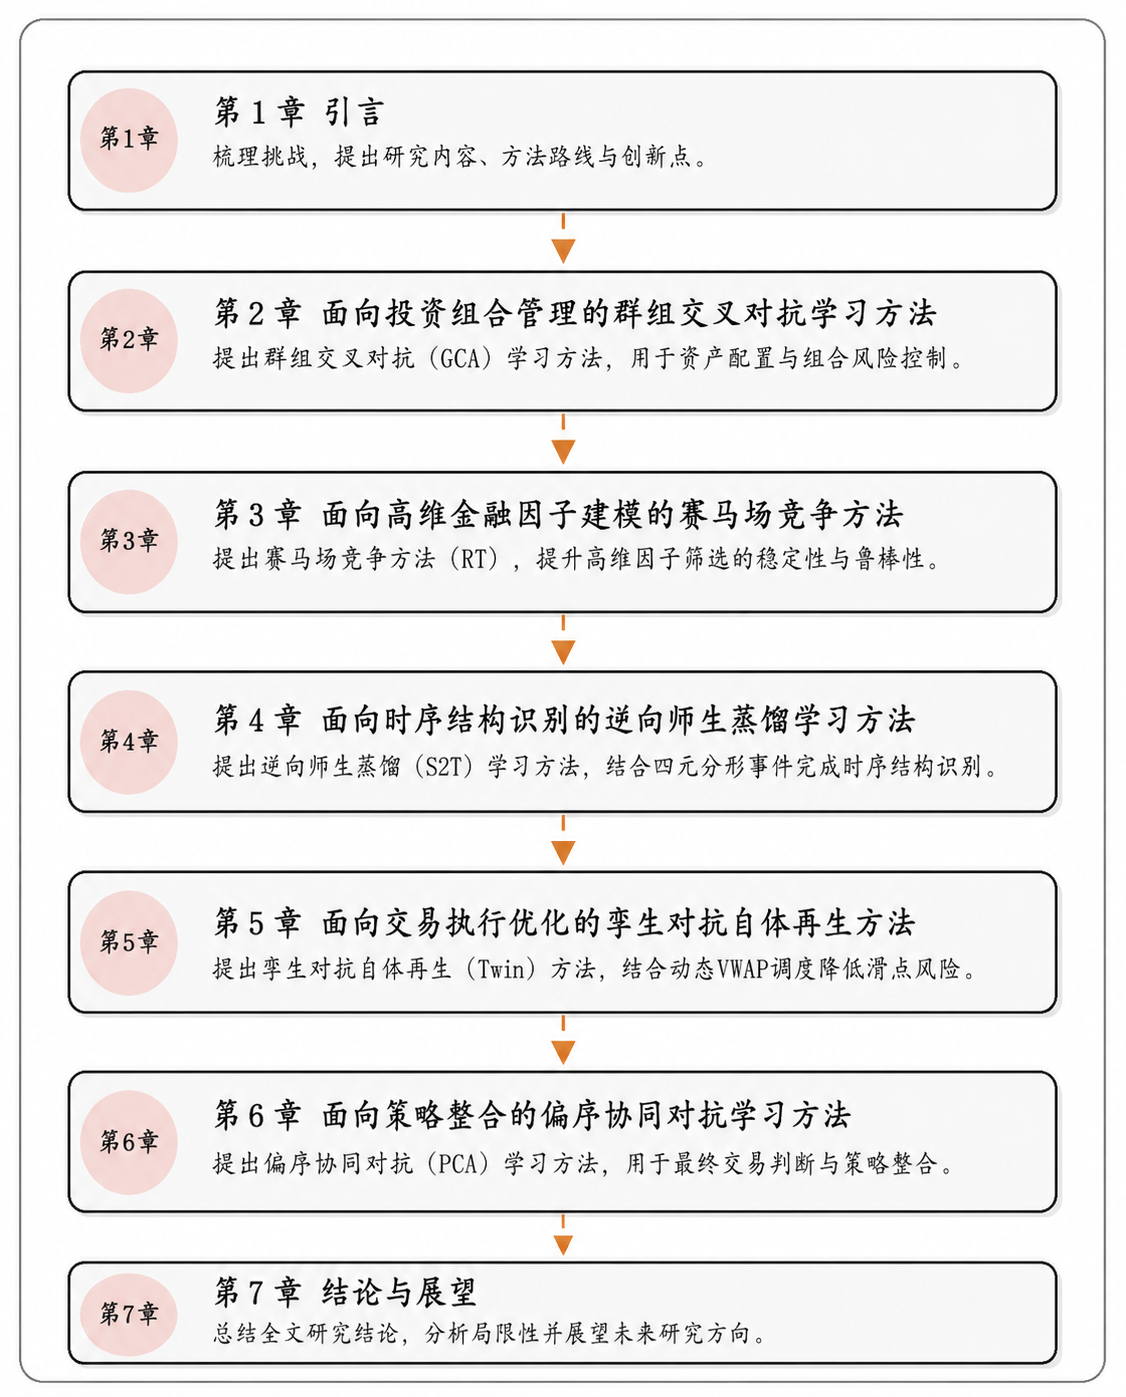
\includegraphics[width=0.95\textwidth]{figures/p1-3.png}
    \caption{本文章节结构与研究内容安排示意图}
    \label{fig:1-3}
\end{figure}

各章内容安排如下：

第1章引言。本章从对冲基金交易的系统性、自动化和博弈性特征出发，说明本文不将交易算法理解为单一价格预测模型，而是将其置于完整交易决策链条中加以讨论。在此基础上，本章梳理投资组合管理、高维金融因子建模、时序结构识别、交易执行优化和策略整合相关工作的研究现状，进一步明确本文的研究内容、方法路线和创新点。

第2章“面向投资组合管理的群组交叉对抗学习方法”。本章面向交易决策链中的资产选择与资金配置环节，重点讨论如何在多个资产之间识别配置对象并形成稳定资金配置。针对单一模型难以稳定刻画多资产相对关系、组合权重容易受噪声扰动以及风险约束难以嵌入配置过程等问题，本章提出群组交叉对抗（GCA）学习方法，通过多智能体群组之间的交叉校验与竞争约束，提高多资产配置中的信号稳定性和组合权重生成能力。

第3章“面向高维金融因子建模的赛马场竞争方法”。本章面向交易决策链中的因子依据形成环节，重点讨论哪些因子能够稳定支撑资产选择。在第2章关注多资产配置关系的基础上，本章进一步讨论高维因子空间中有效信息容易被噪声掩盖、模型容易在局部因子结构上过早收敛的问题。为此，本章提出赛马场竞争方法，通过动态选优、模型替换和成熟—新生模型之间的双向知识迁移，提升高维金融因子表征的稳定性和可解释性。

第4章“面向时序结构识别的逆向师生蒸馏学习方法”。本章面向交易决策链中的时机识别环节，重点讨论当前趋势结构是否具备交易意义。针对金融时间序列中局部噪声、伪结构和结构边界漂移导致交易时机判断不稳定的问题，本章以四元分形事件标注方法完成波浪结构量化表达，并设计逆向师生蒸馏机制，将弱模型中的失败经验反馈给强模型，从而抑制噪声过拟合并提升时序结构识别的稳定性。

第5章“面向交易执行优化的孪生对抗自体再生方法”。本章面向交易决策链中的订单执行环节，重点讨论如何降低滑点、市场冲击和执行偏差，并提升执行路径稳定性。在前序章节形成资产选择、因子依据和结构信号之后，交易信号还需要转化为可执行的订单路径。针对成交量预测误差、流动性错配和局部对抗失衡可能导致理论收益被执行成本侵蚀的问题，本章提出孪生对抗自体再生方法，通过复制—配对—分化和跨组修复机制，构建“预测成交量—执行路径—滑点控制—崩溃修复”的执行优化闭环。

第6章“面向策略整合的偏序协同对抗学习方法”。本章讨论交易决策链末端的最终交易判断形成问题。涨、跌、平等方向输出在这里不再被解释为孤立分类标签，而是对应买入、卖出或持有等交易动作。在问题定义、模型解释和评价口径上，本章承接资产配置、因子依据、结构信号和执行约束，提出偏序协同对抗（PCA）学习方法，用于改善最终判断中的边界稳定性、策略组织能力和跨资产泛化能力。

第7章结论与展望。本章对全文研究成果进行归纳，总结各章方法在交易决策链中的作用与创新点。随后分析当前研究仍存在的局限，并对后续研究方向进行展望。

本文第2章至第6章分别对应对冲基金交易决策链中的五个关键环节。第2章解决多资产配置对象选择与资金配置问题；第3章进一步解释因子依据形成，为资产选择提供稳定因子依据；第4章围绕时序结构识别，为交易时机判断提供方法支撑；第5章围绕交易执行路径优化，将前序交易信号转化为受滑点和市场冲击约束的订单执行路径；第6章则将方向分类结果组织为买入、卖出或持有等最终交易判断，并以偏序协同对抗学习方法完成策略整合。由此，全文形成“资产选择与资金配置—因子依据形成—时序结构识别—订单执行优化—最终交易判断”的递进关系。通过这种安排，本文既避免将五项研究写成互不相干的独立实验，也避免把所有机制压缩为单一总框架，而是在交易流程中为每一章确定相对明确的任务边界和方法作用。
